\begin{footnotesize}
\begin{sffamily}
\begin{singlespacing}

%%%%%%%%%%%%%%%%%%%%%%%%%%%%%%%%%%%
% 1-1
%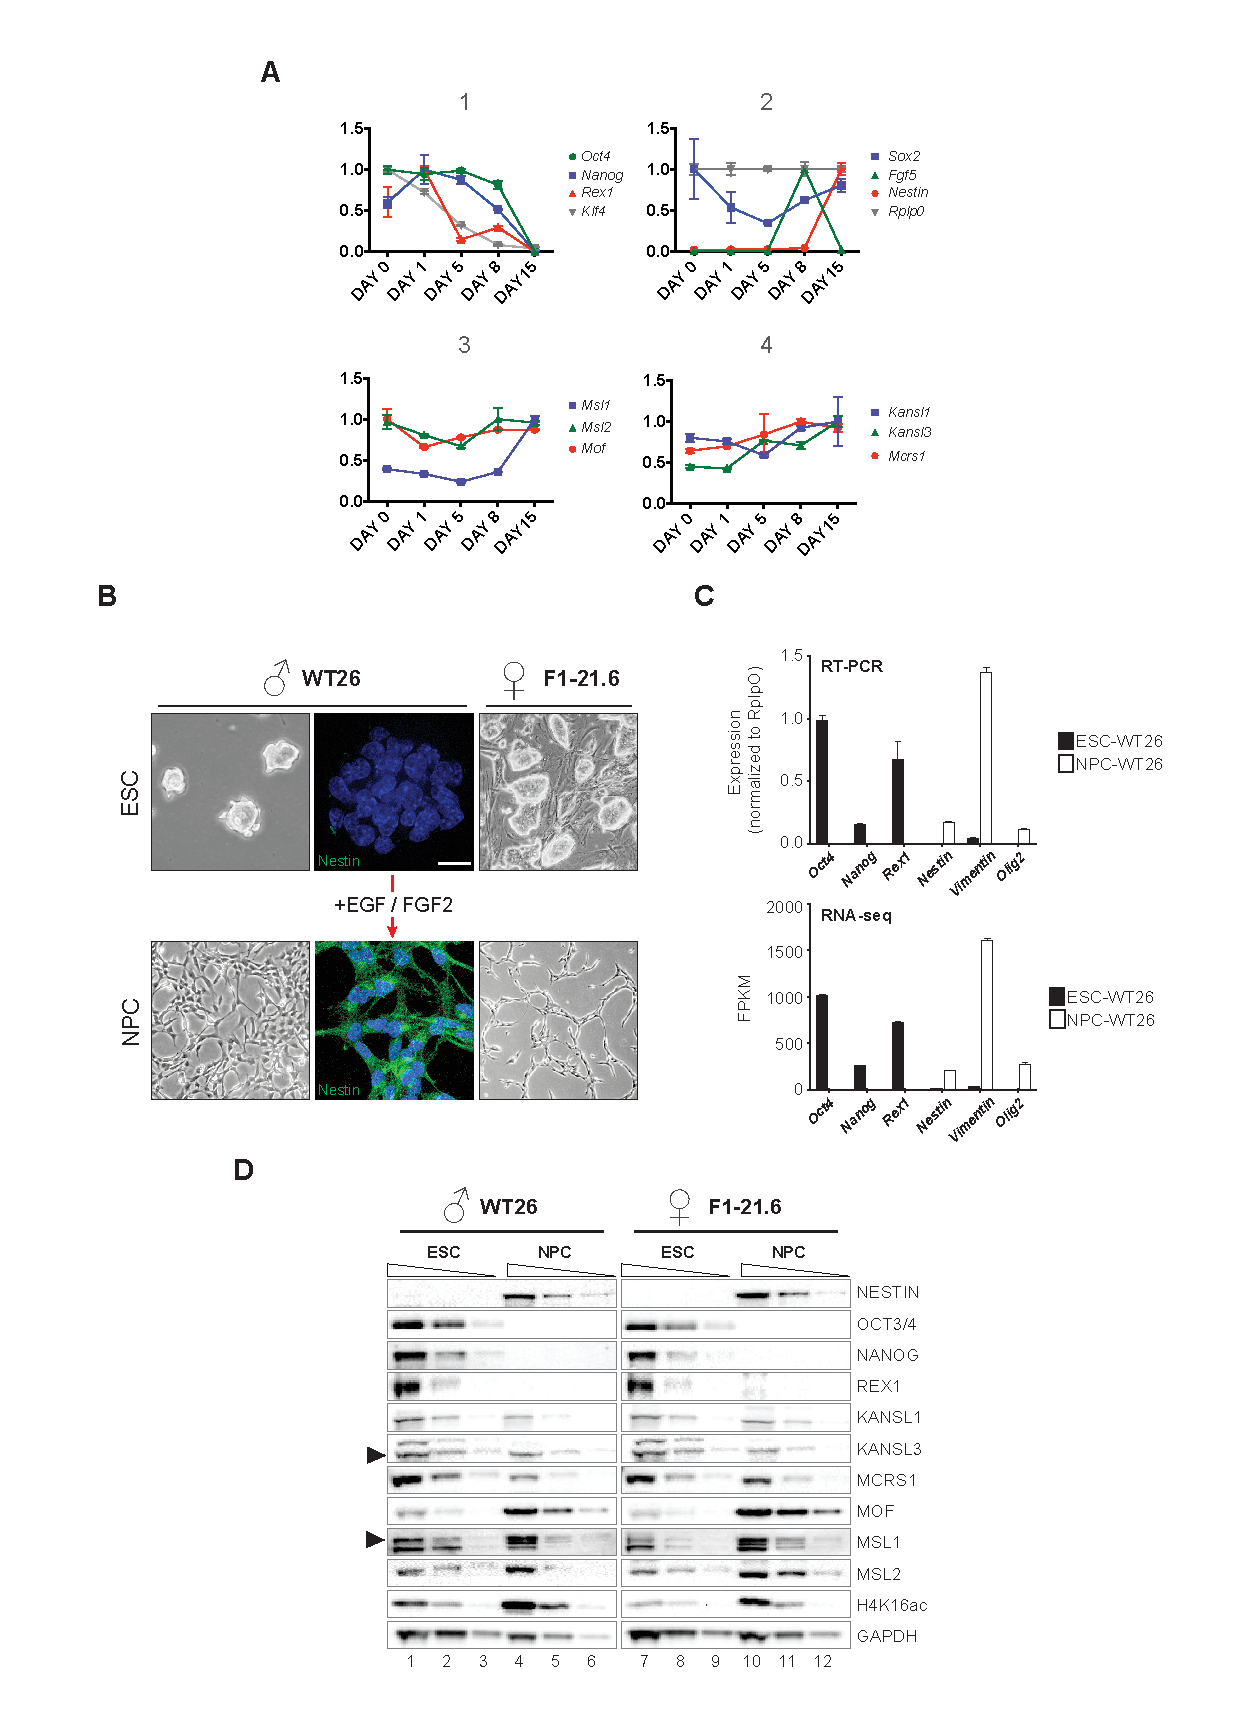
\includepdf[scale=0.9, pages={1}, pagecommand={}, offset=75 -75]{Figures/Appendix/Figure1_supplemental_figure1.pdf}
\textbf{Figure 1—figure supplement 1: Monitoring RNA and protein levels in ESCs and NPCs.
}

A) We monitored the expression dynamics during ESC differentiation for markers of pluripotency (\textit{Oct4, Nanog, Rex1, Klf4}), embryoid body formation (\textit{Fgf5}), differentiation (\textit{Sox2}), and NPC (\textit{Nestin}). Panels 3 and 4 contain the expression profiles for members of the MSL complex (\textit{Msl1, Msl2}), Mof, and the NSL complex (\textit{Kansl1, Kansl3, Mcrs1}), respectively. All results are represented as relative values individually normalized to Rplp0 expression levels (panel 2) on a given day and to the highest expression level of a given gene during the entire differentiation process (highest expression level of each gene = 1). The x-axes show days of differentiation. All results are expressed as means +/- S.D. for technical replicates. For primers see Supplementary File 3C.

(B) Bright field images illustrate the cell morphology before and after the process of differentiation. The im\-mu\-no\-fluo\-res\-cence analysis indicates the specific staining for the NESTIN protein (green) in neuronal progenitors (NPC); DNA is counter\-stained with DAPI (blue).

(C) Expression changes for selected ESC-specific and NPC-specific markers before and after differentiation of wild-type WT26 cells in using RT-PCR analysis and RNA-seq.

(D) Western blots for proteins from two ES cell lines and their NPC derivatives. Different dilutions were loaded (10\%, 30\%, 10\%) with the order indicated on top of the blots. Anti-GAPDH was used as loading control; arrows indicate the protein of interest.

\newpage
%
%%%%%%%%%%%%%%%%%%%%%%%%%%%%%%%%%%%
% 1-2
\begin{minipage}[c]{0.4\textwidth}
\includegraphics{Figures/Appendix/Figure1_supplemental_figure2_scissored.pdf}
%\caption{\label{fig:blue_rectangle} Rectangle}
\end{minipage} \hfill
\begin{minipage}[c]{0.4\textwidth}
\begin{flushleft}
\textbf{Figure 1—figure supplement 2: Verification of antibodies used in this study.}\tabularnewline \tabularnewline
(A) Immunoprecipitations from mouse ESC nuclear extracts with antibodies specific for KANSL1, KANSL3 or MOF and rabbit or rat antisera. The blot was probed with indicated antibodies showing the co-immunoprecipitation of several NSL complex members. Asterisks represent the IgG signal. Pol II = RNA Polymerase II.\tabularnewline \tabularnewline
(B) and (C) same as (A) except that immunoprecipitations were performed with antibodies specific to MSL1 (B) and MSL2 (C). Asterisks represent the IgG signal.
\end{flushleft}
\end{minipage}
\newpage
%%%%%%%%%%%%%%%%%%%%%%%%%%%%%%%%%%%
% 2-1
\includegraphics[width=\textwidth]{Figures/Appendix/Figure2_supplemental_figure1_scissored.pdf}

\textbf{Figure 2—figure supplement: ChIP-seq quality measures.}

(A) Correlation plot for all individual ChIP-seq and input samples from ESCs (left) and NPCs. The genome was sampled in windows of 10 kb length; the numbers of reads per bin were counted for each ChIP sample and correlated using Pearson correlation. The calculation and heatmap visualization were done with the bamCorrelate module from the deepTools suite (Ramirez et al., 2014).

(B) The bar chart depicts the fraction of ChIP-seq peaks for each protein that reside within each cluster shown in Figure 2, i.e. approximately 30\% of MSL1 peaks in ESCs locate in cluster E. Note that the absolute numbers of peaks differ between the samples (see Supplementary file 1B for absolute peak numbers and Methods and Materials for peak calling details).
\newpage
%%%%%%%%%%%%%%%%%%%%%%%%%%%%%%%%%%%
% 3-1
\includegraphics[width=0.77\textwidth]{Figures/Appendix/Figure3_supplemental_figure1_scissored.pdf}

\textbf{Figure 3—figure supplement 1: MSL and NSL complexes target promoters of broadly expressed genes in ESCs and NPCs.
}

(A) The heatmap is related to Figure 3B as it is based on all genes that are bound by at least 1 ChIPed factor in ESCs or NPCs. The intensity of the color depicts the fraction of the 1 kb TSS-region that was covered by a binding site of MOF, MSL1, MSL2, KANSL3 or MCRS1. Rows and columns were sorted using hierarchical clustering on the Euclidean distances of the overlap fractions using R. The left color bar indicates which genes are targeted in 1 or both cell types.

(B) Distribution of expression values from RNA-seq data in ESCs and NPCs for genes targeted by MSL and NSL complex members together or by the NSL complex only. P-values were calculated using Welch t-test.
(C) Results of the GO term analysis using DAVID (Huang da et al., 2009) on genes that were bound at the TSS in ESCs by NSL complex members only or both MSL and NSL complexes.

(D) The pie charts depict how many times annotated TSSs overlapped with a CpG island. The vast majority of genes that were bound in ESCs by MSL and NSL together or by NSL complex members alone overlapped with at least 1 CpG island (dark and medium blue) while approximately 2/3 of the non-target-TSS did not overlap with any CpG island (light blue for 0 CpG islands within the queried regions).
\newpage
%%%%%%%%%%%%%%%%%%%%%%%%%%
% 3-2
\includegraphics[width=\textwidth]{Figures/Appendix/Figure3_supplemental_figure2_scissored.pdf}

\textbf{Figure 3—figure supplement 2: The NSL-, but not the MSL-binding mode of \textit{D.~me\-la\-no\-gas\-ter} is present in mammalian cells.}

(A) Exemplary genome browser snapshots of the X-linked fly gene CG4419. Shown here are the sequencing-depth normalized profiles for ChIP and corresponding input samples, clearly showing a broad enrichment of MOF and MSL1 along the entire gene body in male (m) \textit{D.~me\-la\-no\-gas\-ter} while all other marks show sharp enrichments around the TSS (including MSL1 and MOF in female (f) \textit{D.~me\-la\-no\-gas\-ter}) which are similar to those seen for both complexes in mouse cells (Figure 3A and 3D).

(B) Comparison of expressed (FPKM \textgreater 4) mouse genes whose homologous genes are either bound or not bound by MOF and its complexes in the fly. We extracted the input-normalized ChIP-seq values for 6~kb regions around the TSS using the computeMatrix module of deepTools (Ramirez et al., 2014). H3K4me3 signal is from a published data set, see Supplementary file 2 for the corresponding accession number.
\newpage
%%%%%%%%%%%%%%%%%%%%%%%%%%
% 3-3
\includegraphics[width=\textwidth]{Figures/Appendix/Figure3_supplemental_figure3_scissored.pdf}

\textbf{Figure 3—figure supplement 3: Effects of shRNA-mediated depletion of MOF, MSL1, MSL2, and KANSL3.}

(A) Time course of knockdown experiments. For experimental details see Methods and Materials. Samples for RNA-sequencing and AP staining (see Figure 4—figure supplement 4) were extracted 4~days after puromycin selection of shRNA-treated cells.

(B) Proliferation assay for shRNA-treated cells, starting at day~4 after puromycin selection (see Figure 3---figure supplement 3A).

(C) Bar plots depicting the fractions of genes (per chromosome) that were significantly up- or downregulated in RNA-seq experiments from shRNA-treated cells. The left plot contains genes which were defined as TSS-targets in the respective ChIP-seq samples, the right plot contains genes that were neither classified as TSS- nor as TSS-distal targets. The labels on each bar indicate the chromosome name and the total number of genes that fulfilled the criteria for this chromosome (significantly affected, TSS-bound or non-targeted). See Methods and Materials for details of the classification.
\newpage
%%%%%%%%%%%%%%%%%%%%%%%%%%
% 3-4
\includegraphics[width=\textwidth]{Figures/Appendix/Figure3_supplemental_figure4_scissored.pdf}

\textbf{Figure 3—figure supplement 4: Assessment of ChIP signals around the TSSs of putative target genes as determined by ChIP-seq.}

(A) Genome Browser snapshots of several MSL/NSL (left) or NSL-only (Visel et al.) target genes and respective sequencing-depth-normalized ChIP-seq and input signals from ESCs. The exact genomic coordinates are indicated on top of each panel. Gene names are indicated on the bottom.

(B) ChIP-qPCR validation for MOF (green) and KANSL3 (purple) signals. Im\-mu\-no\-pre\-ci\-pi\-tated DNA was amplified by qPCR with primer sets positioned at the promoter (P) and end (E) of the coding sequence (Supplementary file 3A). Results are expressed as mean +/- S.D. of 3 biological replicates; cells were harvested for experiments on day~4 (\textit{Kansl3}) or 5 (\textit{Mof}) of knockdown.

(C) ChIP-qPCR for MSL1 (blue), MSL2 (red) and KANSL3 (purple) in ESCs treated with sh-RNA (scrambled or against a specific transcript). Signals on genes were evaluated using primers at the promoter (P), and end (E) of the coding sequence. Results are expressed as mean +/- S.D. of 3~bio\-lo\-gi\-cal replicates; cells were harvested for experiments on day~5 of \textit{Mof} knockdown.
\newpage
%%%%%%%%%%%%%%%%%%%%%%%%%%
% 4-1
\includegraphics[width=\textwidth]{Figures/Appendix/Figure4_supplemental_figure1_scissored.pdf}

\textbf{Figure 4—figure supplement 1: MSL2 and KANSL3 show strong enrichments at typical and super enhancers in ESCs.}

(A) Boxplots demonstrating the distribution of mean ChIP enrichments for enhancer regions defined by H3K4me1 and H3K27ac marks in ESCs (see Creyghton et al., 2010 for details) that overlap with the clusters of binding defined by our ChIP-seq samples. Mean values were extracting using the UCSCtool bigWigAverageOverBed.

(B) Summary plots for typical enhancer regions (Whyte et al., 2013) that overlapped with either MSL2 (top) or KANSL3 (bottom) peaks. Different colors indicate different ChIP-seq signals. Related to the heatmaps of Figure 4B.

(C) Genome browser snapshots of sequencing-depth normalized ChIP-seq and input profiles for super enhancers of key pluripotency factors.
\newpage
%%%%%%%%%%%%%%%%%%%%%%%%%%
% 4-2
\includegraphics[width=\textwidth]{Figures/Appendix/Figure4_supplemental_figure2_scissored.pdf}

\textbf{Figure 4—figure supplement 2: MOF is moderately enriched at non-canonical enhancers.}

(A) Summary plots of ChIP-seq values for binding sites belonging to cluster D. The regions were divided based on the presence or absence of annotated ESC enhancers (Whyte et al., 2013, Creyghton et al., 2010).

(B) Heatmaps of ChIP-seq read densities of known enhancer markers for the ESC-specific binding sites of our proteins of interest (cluster D, see Figure 2) and random genomic regions. The binding sites of cluster D (excluding regions with TSSs) were divided into 2 basic groups based on the presence or absence of known ESC enhancers (Whyte et al., 2013, Creyghton et al., 2010). The latter group was further divided into 3 (arbitrarily numbered) sub-clusters based on hierarchical clustering of the values from DNase hypersensitivity sites, p300, H3K4me1 and our MOF sample (in ESCs). Heatmaps of the ESC-enhancer-containing regions were sorted according to p300, those of the sub-clustered regions were sorted according to the MOF signal.

(C) Related to (B), shown here are the corresponding summary plots of ChIP-seq values for cluster D binding sites that do not overlap with annotated enhancer regions (bottom part of the heatmaps in the figure above). The 3~indicated groups are based on the hierarchical clustering that was performed on p300, H3K4me1 and MOF values (``Regions without annotated ESC enhancers'' in (B)).
\newpage
%%%%%%%%%%%%%%%%%%%%%%%%%%
% 4-3
\includegraphics[width=\textwidth]{Figures/Appendix/Figure4_supplemental_figure3_scissored.pdf}

\textbf{Figure 4—figure supplement 3: MSL2 has intergenic binding sites in DNA-hypomethylated regions that are enriched for SMAD3 binding sites.}

(A) We extracted the percentage of methylated CpGs and the input-normalized ChIP-seq values from KANSL3 and MSL2 and 5 kb surrounding the center of the regions belonging to cluster C (Figure 2) and random genomic control regions. All heatmaps were sorted according to the percentages of methylated CpGs (Stadler et al., 2011).

(B) Motif obtained by MEME analysis on the top 200 MSL2 peaks within cluster C.

(C) Same as for (A), except that the score was the motif hit score for SMAD3 for 1 kb. See Methods and Materials for details.
\newpage
%%%%%%%%%%%%%%%%%%%%%%%%%%
% 4-4
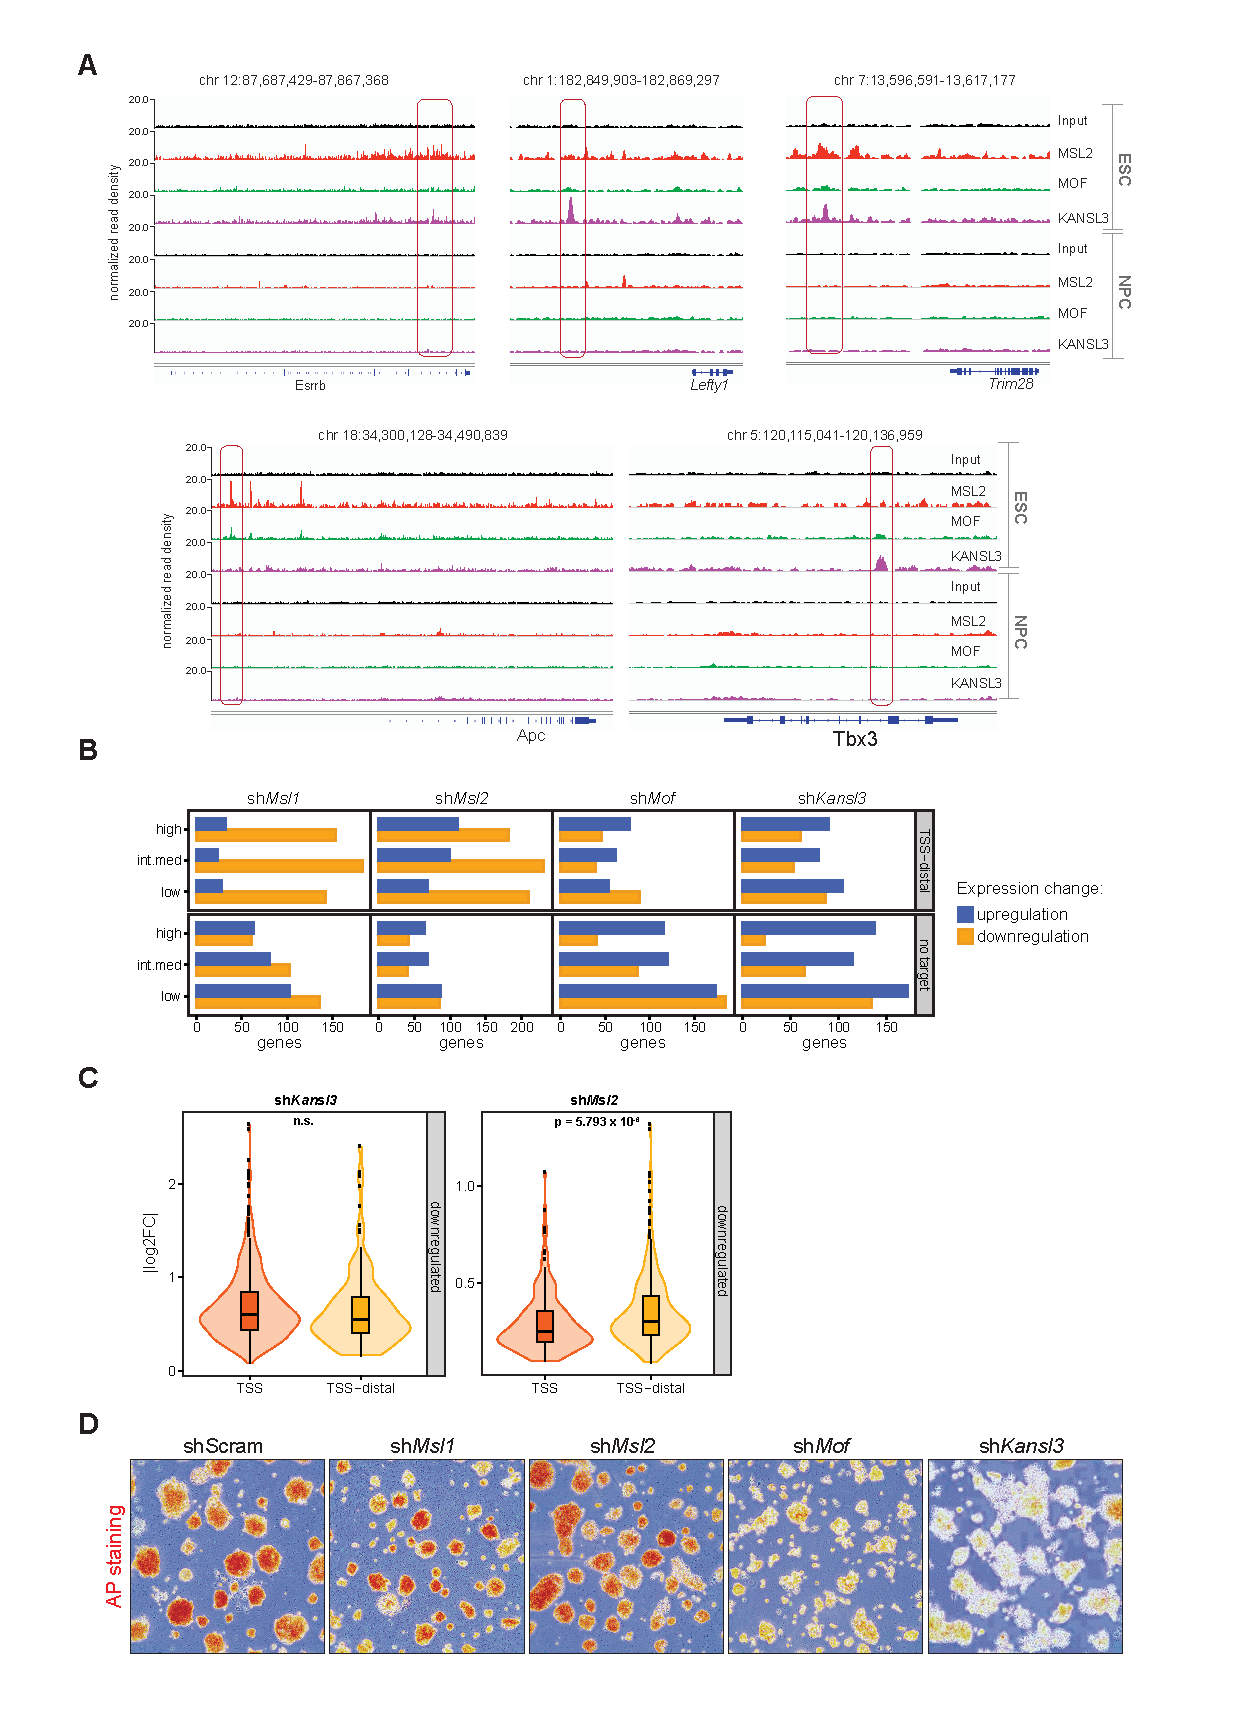
\includegraphics[width=\textwidth]{Figures/Appendix/Figure4_supplemental_figure4.pdf}

\textbf{Figure 4—figure supplement 4: Biological significance of the TSS-distal binding sites of the investigated proteins.}
\newpage

(A) Genome browser snapshots of sequencing-depth normalized ChIP-seq and input profiles. Pink boxes mark the regions cloned and transfected into ESCs and NPCs for luciferase assays (Figure 4D).

(B) Genes that were significantly up- or downregulated in the respective shRNA-treatments compared to shScrambled were classified according to ChIP-seq peak overlaps (TSS-distal, no target) and expression strength in wild type ESCs (high, intermediate, low). See Methods and Materials for details of the classifications.

(C) Distribution of absolute log2 fold changes (shKansl3 or shMsl2 compared to shScrambled) for significantly downregulated genes. Different shades of orange indicate different target classes based on ChIP-seq experiments for KANSL3 or MSL2, respectively. P-values were calculated with Welch t-test.

(D) Alkaline phosphatase staining and morphology of ESC colonies in indicated knockdowns after 4 days growth under puromycin selection (see Figure 3—figure supplement 3A). MOF- and KANSL3-depleted cells demonstrate reduced alkaline phosphatase positive colonies with increased differentiation compared with MSL1- and MSL2-depleted cells and scrambled control.
\newpage
%%%%%%%%%%%%%%%%%%%%%%%%%%
% 5-1
\includegraphics[width=0.9\textwidth]{Figures/Appendix/Figure5_supplemental_figure1_scissored.pdf}

\textbf{Figure 5—figure supplement 1: The MSL proteins bind to multiple loci within the X inactivation center (XIC).}

(A) Genome browser snapshots of the mouse XIC (top panel) with three enlargements on Jpx, Ftx and Rnf12 genes (lower panels). Red boxes with corresponding numbers mark the enlarged regions presented in the lower panels. The exact genomic coordinates are indicated on top of each panel, arrows represent genes. The signals shown are the sequencing-depth normalized ChIP-seq profiles in NPCs.

(B) ChIP analysis of MSL1, MSL2 and MOF across the DXPas34 mini\-sat\-el\-lite in female ESCs. The x-axis labels indicate the genomic coordinates corresponding to the arrowheads in Figure 5A. The y-axes show the percentage of ChIP recovery for MSL1 and MSL2 (left-hand side) and MOF (right-hand side) normalized to input. For all ChIP experiments, 3~biological replicates were used; all results are expressed as mean +/- S.D.
\newpage
%%%%%%%%%%%%%%%%%%%%%%%%%%
% 6-1
\includegraphics[width=0.9\textwidth]{Figures/Appendix/Figure6_supplemental_figure1_scissored.pdf}

\textbf{Figure 6—figure supplement 1: Cells depleted of MSL1 or MSL2, but not MOF show loss of DXPas34 foci.}

(A) RNA-FISH for \textit{Huwe1} RNA (red) and \textit{DXPas34} RNA (green) in shScrambled-, sh\textit{Msl1}-, sh\textit{Msl2}- and sh\textit{Mof}-treated female ESCs. Shown here are examples of RNA-FISH signals for multicellular colonies and loss of \textit{DXPas34} signal in MSL1- and MSL2-depleted cells. White boxes indicate cells enlarged and resented in Figure 6B. For all experiments, nuclei were coun\-ter\-stained with DAPI (blue).

(B) Summary of RNA-FISH for \textit{DXPas34} and \textit{Huwe1}. Red dots indicate the number of X chromosomes and green dots, \textit{DXPas34} foci (smaller dot = reduced signal). Phenotypes that we observed in knockdowns are categorized into 4 groups containing cells with equal \textit{Huwe1/DXPas34} ratio and with \textit{DXPas34} loss. The percentages indicate how many cells per population showed the respective phenotype.

(C) Corresponding to Figure 6B. Summary of total cell counts from RNA-FISH for (\textit{DXPas34}) and \textit{Huwe1} in MSL1-, MSL2- or MOF-depleted female ESCs.

(D) Gene expression analysis for the indicated genes in female ESCs treated with scrambled RNA (shScram) or shRNA against \textit{Mof}, \textit{Msl1} and \textit{Msl2}. All results are represented as relative values normalized to expression levels in shScram (normalized to \textit{Hprt}) and expressed as means +/- S.D. in 3~biological replicates.

(E) Gene expression analysis for genes of the XIC in female ESCs treated with scrambled RNA or shRNA against \textit{Msl1}, \textit{Msl2} or \textit{Mof}. All results are represented as relative values normalized to expression levels in shScrambled (normalized to \textit{Hprt}) and expressed as means +/- S.D. for 3~biological replicates.
\newpage
%%%%%%%%%%%%%%%%%%%%%%%%%%
% 7-1
\includegraphics[width=.85\textwidth]{Figures/Appendix/Figure7_supplemental_figure1_scissored.pdf}

\textbf{Figure 7—figure supplement 1: Depletion of MSL1 and MSL2 leads to occasional accumulation and spreading of Xist in undifferentiated ESCs.}

(A) RNA-FISH for \textit{Huwe1} RNA (red) and \textit{Xist} RNA (green) in shScrambled- (top left) and sh\textit{Mof}- (top right), sh\textit{Msl1}- (bottom left) and sh\textit{Msl2}-treated (bottom right) female ESCs. Shown here are additional examples of RNA-FISH for multicellular colonies and individual cells exhibiting \textit{Xist}-mediated coating (see Figure 7A). White boxes indicate cells enlarged in Figure 7A. White arrows denote \textit{Huwe1} and \textit{Xist} foci. Dashed lines indicate nuclei borders. For all experiments, nuclei were coun\-ter\-stained with DAPI (blue).

(B) Summary of RNA-FISH for \textit{Xist} and \textit{Huwe1}. The number of green dots indicates the number of X chromosomes within the cell while the larger dot indicates \textit{Xist} accumulation. Cells were classified into three phenotypic groups with cells showing sharp, localized \textit{Xist} signals (once or twice) or \textit{Xist} ``clouds''. The percentages indicate how many cells per population showed the respective phenotype.

(C) Corresponding to Figure 7A. Summary of the total cell counts from \textit{Xist} and \textit{Huwe1} RNA-FISH in indicated knockdowns.
\newpage
%%%%%%%%%%%%%%%%%%%%%%%%%%
% 7-2
\includegraphics[width=\textwidth]{Figures/Appendix/Figure7_supplemental_figure2_scissored.pdf}

\textbf{Figure 7—figure supplement 2: Depletion of MSL1 and MSL2 lead to enhanced Xist accumulation in differentiating ESCs.}

(A) RNA-FISH for \textit{Huwe1} RNA (red) and \textit{Xist} RNA (green) in shScrambled-, sh\textit{Msl1}- and sh\textit{Msl2}-treated differentiating (DAY3) female ESCs. Shown here are additional examples of RNA-FISH for multicellular colonies (see Figure 7C). Dashed lines indicate nuclei borders. For all experiments, nuclei were coun\-ter\-stained with DAPI (blue).

(B) Corresponding to Figure 7C-E. Summary of the total cell counts from \textit{Xist} RNA-FISH in indicated knockdowns. Percentage of cells with respective phenotype indicated in red.

%===============================
\end{singlespacing}
\end{sffamily}
\end{footnotesize}
